\documentclass{article}
\usepackage{amsmath,amssymb}
\usepackage{algorithm}
\usepackage[noend]{algorithmic}
\usepackage{parskip}
\usepackage{url}
\usepackage{amsthm}
\usepackage{graphicx}
\usepackage{subfigure}

\newcommand{\addpicture}[4]
{ \begin{figure}[H] \centering \includegraphics[#1]{figures/#2} \caption{#4} \label{#3}  \end{figure} }

\title{On Range-1-Query (R1Q) Problem}
\date{}
\begin{document}
\maketitle
\section{Introduction}
Range query has wide applications in database systems. There are
roughly two classes of range query, dynamic range query and static range
query. Dynamic range query allows dynamic INSERT and / or DELETE elements,
while the static version allows a preprocessing before answering any
online query.  This paper studies only static range query problem and
adopts the arithmetic model which only counts the number of arithmetic
operation and ignores the operations of memory access.

If the arithmetic operation is general partial sum, a near-linear algorithm of $(O(N \alpha N), O(\alpha N))$ ((preprocessing bound, query bound) for $1$-D array is known \cite{yao}. Chazelle and Rosenberg~\cite{chazelle} have extended it to multi-dimensional array with similar near-linear bound. If the arithmetic operation is
$\min$ or $\max$, by exploiting Four-Russian trick, one can further reduce the preprocessing bound to linear $O(N)$. However, no previous results or work have ever explored the possibility of sub-linear space in some special case.  A sub-linear space preprocessing algorithm does not only reduce the preprocessing complexity, it also reduce possible cache complexity simply by using less memory.

This paper discusses such a special case - {R1Q}, i.e. Range 1-bit Query problem, with the arithmetic operation to be bit-wise and / or. We not only explored the orthogonal (rectangular) {R1Q}, but also non-orthogonal versions.  For the {R1Q} problem, even the exact algorithm can be sub-linear in $1$-D case. If we can tolerate some errors, the
space complexity of the preprocessing algorithm can be further reduced.

Range searching is one of the most important problems in Computational Geometry. Many geometric problems can be modeled as range searching problems. Other applications include Geographical Information Systems (GIS), Computer Graphics, Computed Aided Design (CAD), Spatial Databases and Time Series Databases. It encompasses different types of problems like range counting, range reporting, emptiness queries and optimization queries. Range searching has been extensively studied in literature \cite{sharir, agarwal, ishaque}.

Emptiness queries is one of the important problem types in range searching \cite{erickson}. Till now, the major focus has been towards finding whether a given shape is empty or not in $R^d$. For the first time, we consider the emptiness problem for $Z^d$ i.e for an integer lattice. We name this problem as Range-1-Query (R1Q) problem.

The R1Q problem is defined as follows. Given a bit vector $A[1 \ldots n]$ and indices $i$ and $j$ such that $1 \le i \le j \le n$, find efficiently if there exists a 1 in the subarray $A[i, j]$. We usually represent it as $R1Q(i, j)$. In this paper, we present an efficient approximation algorithm to answer the range queries in constant time with very less extra memory. We also extend the algorithm to solve the problem in higher dimensions.

The R1Q problem is closely related to Range Minimum Query (RMQ) problem. Given an array $A[1 \ldots n]$ and indices $i$ and $j$, the range minimum query denoted as $RMQ(i, j)$ asks us to find the position of the minimum element in the subarray $A[i, j]$.

As no good algorithms have been developed for R1Q, we focus our attention to RMQ and survey a few existing algorithms for the same. A good survey of RMQ algorithms is given in \cite{website:danielp}. For each of the algorithms we give the complexity of the algorithm as a 3-tuple in the form (ExtraSpaceInBits, PreprocessTime, QueryTime).

\subsection{Scan Algorithm}
We simply scan the array $A$ from index $i$ to $j$ and find the minimum element.\\
Complexity $= (\mathcal{O}(1), \mathcal{O}(1), \mathcal{O}(n))$   

\begin{algorithm}
\begin{algorithmic}[1]
\caption{: \textsc{RMQ-Scan}($start$, $end$)}
\medskip
\STATE $min \gets start$
\medskip
\FOR{$i \gets start+1$ to $end$}
	\IF{$A[i] < A[min]$}
		\STATE $min \gets i$
	\ENDIF
\ENDFOR
\medskip
\RETURN $min$
\medskip
\end{algorithmic}
\end{algorithm}

\subsection{Query Table (QT)}
The array $A$ is preprocessed and a table called \textit{Query Table}, $M$, is created which stores the range minimum for all $\mathcal{O}(n^2)$ possible range queries. Each element of the query table, $M[i][j]$, stores the position of the minimum element in the subarray $A[i \ldots j]$ which is found by scanning over the range. For any given query, we just find the value at $M[i][j]$.

Complexity $= (\mathcal{O}(n^2 \log(n)), \mathcal{O}(n^3), \mathcal{O}(1))$

\begin{algorithm}
\begin{algorithmic}[1]
\caption{: \textsc{RMQ-QT-Preprocess}()}
\medskip
\FOR{$i \gets 1$ to $n$}
	\FOR{$j \gets i$ to $n$}
		\STATE $M[i][j] \gets $ \textsc{RMQ-Scan}($i$, $j$)
	\ENDFOR
\ENDFOR
\medskip
\RETURN $M$
\medskip
\end{algorithmic}
\end{algorithm}

\begin{algorithm}
\begin{algorithmic}[1]
\caption{: \textsc{RMQ-QT}($start$, $end$)}
\medskip
\RETURN $M[start][end]$
\end{algorithmic}
\end{algorithm}

\subsection{Query Table (QT): Dynamic Programming (DP)}
The algorithm is almost same as the Query Table algorithm except while finding the range minimum during preprocessing, we use dynamic programming. That is, we find $M[i][j]$ using $M[i][j-1]$ and $a[j]$ as shown below. Using DP, we can reduce the preprocessing time by a factor of $n$.

Complexity $= (\mathcal{O}(n^2 \log(n)), \mathcal{O}(n^2), \mathcal{O}(1))$

\begin{algorithm}
\begin{algorithmic}[1]
\caption{: \textsc{RMQ-QTDP-Preprocess}()}
\medskip
\FOR{$i \gets 1$ to $n$}
	\STATE $M[i][i] \gets i$
\ENDFOR
\medskip
\FOR{$i \gets 1$ to $n-1$}
	\FOR{$j \gets i+1$ to $n$}
		\IF{$A[j] < A[M[i][j-1]]$}
			\STATE $M[i][j] \gets j$
		\ELSE
			\STATE $M[i][j] \gets M[i][j-1]$
		\ENDIF
	\ENDFOR
\ENDFOR
\medskip
\RETURN $M$
\medskip
\end{algorithmic}
\end{algorithm}

\begin{algorithm}
\begin{algorithmic}[1]
\caption{: \textsc{RMQ-QTDP}($start$, $end$)}
\medskip
\RETURN $M[start][end]$
\medskip
\end{algorithmic}
\end{algorithm}

\subsection{Chunks Algorithm}
The array $A$ is divided into $\sqrt n$ chunks, each of which will be of size $\sqrt n$. For simplicity, we can assume the $n$ is a perfect square. Maintain an array $M$ of size $\sqrt n$, where each element $M[k]$ stores the position of the minimum element in the $k$\textsuperscript{th} chunk. To find the position of the minimum element in subarray $A[i \ldots j]$, we have to make use of at most three subranges:
\begin{itemize}
\item The partial chunk, from $i$ to the start of the first innermost chunk
\item All complete chunks in the range from $i$ to $j$
\item The partial chunk, from the end of the last innermost chunk to $j$
\end{itemize}

Complexity $= (\mathcal{O}(\sqrt n \log(n)), \mathcal{O}(n), \mathcal{O}(\sqrt n))$

\begin{algorithm}
\begin{algorithmic}[1]
\caption{: \textsc{RMQ-Chunks-Preprocess}()}
\medskip
\FOR{$i \gets 1$ to $\sqrt n$}
	\STATE $min \gets \sqrt n (i-1) + 1$
	\FOR{$j \gets \sqrt n (i-1) + 1$ to $\sqrt n \cdot i - 1$}
		\IF{$A[j] \le A[min]$}
			\STATE $min \gets j$
		\ENDIF
	\ENDFOR
	\medskip
	\STATE $M[i] \gets min$
\ENDFOR
\medskip
\RETURN $M$
\medskip
\end{algorithmic}
\end{algorithm}

\begin{algorithm}
\begin{algorithmic}[1]
\caption{: \textsc{RMQ-Chunks}($start$, $end$)}
\medskip
\STATE $min \gets start$
\STATE $chunkstart \gets \lceil {start \over \sqrt n} \rceil$
\STATE $chunkend \gets \lfloor {end \over \sqrt n} \rfloor$
\medskip
\FOR{$i \gets start+1$ to $\sqrt n \cdot chunkstart$}
	\IF{$A[i] < A[min]$}
		\STATE $min \gets i$
	\ENDIF
\ENDFOR
\FOR{$i \gets chunkstart$ to $chunkend$}
	\IF{$M[i] < A[min]$}
		\STATE $min \gets M[i]$
	\ENDIF
\ENDFOR
\FOR{$i \gets \sqrt n \cdot chunkend$ to $end$}
	\IF{$A[i] < A[min]$}
		\STATE $min \gets i$
	\ENDIF
\ENDFOR
\medskip
\RETURN $min$
\medskip
\end{algorithmic}
\end{algorithm}

\subsection{Sparse Table (ST)}
The algorithm is given in \cite{benderetal}. The array $A$ is preprocessed and a table called \textit{Sparse Table}, $M$, of size $n \log(n)$ is created. The element $M[i][j]$ stores the position of the minimum element in the subarray $A[i \ldots (i+2^j-1)]$. To answer the range query, divide the range $[i, j]$ into two subranges which entirely cover the range and find the range minimum from the two. Both the subranges will be of size $2^{\lfloor \log(j-i+1) \rfloor}$, but, one subrange starts at $i$ and the other ends at $j$. 

Complexity $= (\mathcal{O}(n \log^2(n)), \mathcal{O}(n \log(n)), \mathcal{O}(1))$

\begin{algorithm}
\begin{algorithmic}[1]
\caption{: \textsc{RMQ-ST-Preprocess}()}
\medskip
\FOR{$i \gets 1$ to $n$}
	\STATE $M[i][0] \gets i$
\ENDFOR
\medskip
\FOR{$j \gets 1$ to $\lfloor \log(n) \rfloor$}
	\FOR{$i \gets 1$ to $n-2^j+1$}
		\IF{$A[M[i][j-1]] < A[M[i+2^{j-1}-1][j-1]]$}
			\STATE $M[i][j] \gets M[i][j-1]$
		\ELSE
			\STATE $M[i][j] \gets M[i+2^{j-1}-1][j-1]$
		\ENDIF
	\ENDFOR
\ENDFOR
\medskip
\RETURN $M$
\medskip
\end{algorithmic}
\end{algorithm}

\begin{algorithm}
\begin{algorithmic}[1]
\caption{: \textsc{RMQ-ST}($start$, $end$)}
\label{sparsetable}
\medskip
\STATE $k \gets \lfloor \log (end-start+1) \rfloor$
\STATE $min \gets 0$
\medskip
\IF{$A[M[start][k]] \le A[M[end-2^k+1][k]]$}
	\STATE $min \gets M[start][k]$
\ELSE
	\STATE $min \gets M[end-2^k+1][k]$
\ENDIF
\medskip
\RETURN $min$
\medskip
\end{algorithmic}
\end{algorithm}

\subsection{Segment Trees}
The array $A$ is preprocessed and a segment tree is built for it. A segment tree is a heap like data structure where each node represents an interval or a segment.

The segment tree for the interval or range $[l, r]$ is recursively defined as:
\begin{enumerate}
\item The node for $[l, r]$ holds the information for the interval. In RMQ problem, the node stores the position of the minimum element in the interval.
\item If $l < r$, then the node $[l, r]$ will have two children
\begin{enumerate}
\item Left child with interval $[l, \lfloor (l+r)/2 \rfloor]$
\item Right child with interval $[\lfloor (l+r)/2 \rfloor + 1, r]$
\end{enumerate}
\end{enumerate}

The height of the segment tree is $\lfloor \log n \rfloor + 1$. Store the information of each of the nodes of the segment tree in an array $M$, of size $2^{\lfloor \log n \rfloor + 2}$, where each element $M[i]$ stores the position of the minimum element for the  $i^{th}$ node. To answer $RMQ(i, j)$ we split $[i, j]$ as
\begin{align*}
[i, j] = [i, p_1] + [p_1+1, p_2] + [p_2 + 1, p_3] + \cdots + [p_m+1, j]
\end{align*}
such that the intervals $[i, p_1], [p_1+1, p_2], \ldots, [p_m+1, j]$ are present in the segment tree and the position of the minimum element for all these intervals are stored in $M$. The query can be answered by finding the minimum element among all these intervals and taking their minimum. Any interval can be split down into $\mathcal{O}(\log (n))$ segment tree intervals. Hence, answering the query takes $\mathcal{O}(\log (n))$ time.

Complexity $= (\mathcal{O}(n \log(n)), \mathcal{O}(n), \mathcal{O}(\log (n)))$

\begin{algorithm}
\begin{algorithmic}[1]
\caption{: \textsc{RMQ-SegT-Preprocess}()}
\medskip
\FOR{$i \gets 0$ to $n-1$}
	\STATE $M[i] \gets -1$
\ENDFOR
\medskip
\STATE \textsc{RMQ-SegT-Initialize($1, 0, n-1$)}
\medskip
\RETURN $M$
\medskip
\end{algorithmic}
\end{algorithm}

\begin{algorithm}
\begin{algorithmic}[1]
\caption{: \textsc{RMQ-SegT-Initialize}($i, low, high$)}
\medskip
\IF{$low = high$}
	\STATE $M[i] \gets low$
	\RETURN
\ENDIF
\medskip
\STATE \textsc{RMQ-SegT-Initialize($2i, low, \left( {low + high \over 2} \right)$)}
\STATE \textsc{RMQ-SegT-Initialize($2i + 1, \left( {low + high \over 2} + 1 \right), high$)}
\medskip
\IF{$A[M[2i]] \le A[M[2i+1]]$}
	\STATE $M[i] = M[2i]$
\ELSE
	\STATE $M[i] = M[2i+1]$
\ENDIF
\medskip
\RETURN
\medskip
\end{algorithmic}
\end{algorithm}

\begin{algorithm}
\begin{algorithmic}[1]
\caption{: \textsc{RMQ-SegT}($i, low, high, start, end$)}
\medskip
\STATE \textbf{Function call:} \textsc{RMQ-SegT}($1, 0, n-1, start, end$)
\medskip
\IF{$start > high$ or $end < low$}
	\RETURN -1
\ENDIF
\IF{$low \ge start$ and $high \le end$}
	\RETURN $M[i]$
\ENDIF
\medskip
\STATE $lmin \gets $ \textsc{RMQ-SegT}($2i, low, \left( {low + high \over 2} \right), start, end$)
\STATE $rmin \gets $ \textsc{RMQ-SegT}($2i+1, \left( {low + high \over 2} + 1 \right), high, start, end$)
\medskip
\IF{$lmin = -1$}
	\STATE $min \gets rmin$
\ELSIF{$rmin = -1$}
	\STATE $min \gets lmin$
\ELSIF{$A[lmin] \le A[rmin]$}
	\STATE $min \gets lmin$
\ELSE
	\STATE $min \gets rmin$
\ENDIF
\medskip
\RETURN $min$
\medskip
\end{algorithmic}
\end{algorithm}

\subsection{Berkman Vishkin Algorithm}
The core ideas of the algorithm are from previous works \cite{gabowtarjan} and \cite{gabowbentley}. The presentation combines the ideas given in \cite{berkmanvishkin} and \cite{gabowbentley}. The presentation is closely followed from \cite{bendercolton} and \cite{fischerheun}. A cartesian tree C, of an array $A$ is a binary tree. The root of the tree is the minimum element of the array and it stores the position of the minimum element. The left and right children are recursively constructed. The tree can be built in $\mathcal{O}(n)$ time.

The cartesian tree for the range $A[l, r]$ is recursively defined as:
\begin{enumerate}
\item The root is the minimum element in the range $[l, r]$ and labeled with the position of the minimum element in the range.
\item If $l < r$, then the node $[l, r]$ will have two children
\begin{enumerate}
\item Left child with interval $[l, \lfloor (l+r)/2 \rfloor]$
\item Right child with interval $[\lfloor (l+r)/2 \rfloor + 1, r]$
\end{enumerate}
\end{enumerate}

Three arrays $E, H, R$ are created to store the information of the cartesian tree.
\begin{enumerate}
\item $E[1 \ldots 2n-1]$ stores the labels of visited nodes in the Eulerian tour
\item $H[1 \ldots 2n-1]$ stores the heights of the corresponding visited nodes
\item $R[1 \ldots n]$ stores the first occurrence of $A[i]$ in the Euler tour
\end{enumerate}

We now answer the range query using the formula\\
$RMQ_A(i, j) = E[\pm RMQ_H(R[i], R[j])]$

We solve $\pm RMQ_H(R[i], R[j])$ as follows. Let $N = 2n-1$. The array $H[1 \ldots N]$ is partitioned into blocks of size $\frac{\log N}{2}$. Define two arrays $A^\prime$ and $B$ such that
\begin{enumerate}
\item $A^\prime[1 \ldots \frac{2N}{\log N}]$ stores the minimum element in different blocks
\item $B[1 \ldots \frac{2N}{\log N}]$ stores the position of the minimum element in different blocks
\end{enumerate} 

The array $A^\prime$ is preprocessed using ST algorithm. Answering range queries in $A^\prime$ has the complexity in extra space and query time as ($\mathcal{O}(N), \mathcal{O}(1)$). The array $A^\prime$ should also be preprocessed to answer queries in a single block. There are $\frac{2N}{\log N}$ blocks each of size $\frac{\log N}{2}$. Also, the array $H$ has the special property of adjacent elements differing by 1. In that case, all the $\frac{2N}{\log N}$ blocks can be mapped to $\mathcal{O}(\sqrt N)$ normalized blocks. For each normalized block, all possible RMQs are precomputed and stored in a table. An array $R[1 \ldots \frac{2N}{\log N}]$ is used to map each of the blocks to a normalized block. To answer $\pm RMQ(i, j)$, we compute:
\begin{enumerate}
\item The minimum from $i$ to the end of its block
\item The minimum of inner complete blocks between $i$ and $j$
\item The minimum from starting of $j$'s block to $j$
\end{enumerate} 

The position of the minimum of the three values is returned as the answer. All the three minimums can be found in constant time. The second minimum is found through the preprocessing done to array $A^\prime$. The first and the third minimum can be found by identifying the normalized blocks they map to and then finding the RMQ for the particular ranges in those normalized blocks.

Complexity $= (\mathcal{O}(n), \mathcal{O}(n), \mathcal{O}(1))$

\section{Proposed Algorithm: Exact}
In this section, we propose a sublinear space, constant time algorithm to solve R1Q problem. The algorithm works for higher dimensions as well.

\subsection{One Dimensional R1Q}
For 1-D R1Q, the input is a linear array $A[1 \ldots n]$. The query R1Q($i, j$) should answer the question as to whether there exists a 1 in the subarray $A[i \ldots j]$.

\subsubsection{Preprocessing}
Partition the array $A[1 \ldots n]$ into $\frac{n}{2^p}$ blocks, each of size $2^p$ where $p$ varies from $\log l$ to $\log n$. For simplicity, set $l = \frac{\log n}{2}$. For each value of $p$, we define two arrays
\begin{itemize}
\item $L[1 \ldots \frac{n}{2^p}]$, where $L[i]$ holds the distance of the position where the first 1 appears from the start of the $i$\textsuperscript{th} block when the block size is $2^p$
\item $R[1 \ldots \frac{n}{2^p}]$, where $R[i]$ holds the distance of the position where the first 1 appears from the end of the $i$\textsuperscript{th} block when the block size is $2^p$
\end{itemize}

The arrays $L$ and $R$ will be used to answer inter-block queries. A data structure to answer the intra-block/in-block queries is still needed. We use the Four Russians trick to compute the intra-block queries. That is, for each of the blocks we maintain a query table where the answers for all possible in-block range queries would be stored. 

For a block size of $l = \frac{\log n}{2}$, there are $2^l = 2^{\frac{\log n}{2}} = \sqrt n$ unique blocks. These are called normalized blocks. For more details on normalized blocks, refer \cite{bendercolton}. For each normalized block $i$, we find the answers for all possible range queries and store in a table $T[i]$.
 
\begin{algorithm}
\begin{algorithmic}[1]
\caption{: \textsc{R1Q-Preprocess}()}
\label{r1qtlrpreprocess}
\medskip
\STATE $l \gets \frac{\log n}{2}$
\medskip
\STATE // For intra-block queries
\FOR {$i \gets 1$ to $\frac{n}{2^l}$}
	\STATE $T[i] \gets $ query table for $i$\textsuperscript{th} block
\ENDFOR
\medskip
\STATE // For inter-block queries
\FOR {$p \gets \log l$ to $\log n$}
	\FOR {$i \gets 1$ to $\frac{n}{2^p}$}
		\STATE $L[p][i] \gets $ distance where first 1 occurs from $i$\textsuperscript{th} block's start
		\STATE $R[p][i] \gets $ distance where first 1 occurs from $i$\textsuperscript{th} block's end
	\ENDFOR
\ENDFOR
\medskip
\RETURN $T$, $L$, $R$
\medskip
\end{algorithmic}
\end{algorithm}

\subsubsection{Query Execution}
To answer the query R1Q($i, j$), we consider two cases as given in Algorithm \ref{r1qtlr}:
\begin{enumerate}
\item If the query $(i, j)$ falls in the same block, we answer the query by a lookup for the particular block. We find the index of the normalized block for the range and using the Four Russians trick, we answer the query
\item If the query $(i, j)$ falls in different blocks, we find two overlapping blocks that completely cover the range and then compute the answer from the two queries
\end{enumerate}

When the query $(i, j)$ are in different blocks, the range query is answered as follows. Let $2^p$ be the largest power of 2 present in the range. Then $p = \lfloor \log (j-i+1) \rfloor$. At this point, we find whether 1 exists in any of the two blocks: $A[i \ldots i+2^p-1]$ and $A[j-2^p+1 \ldots j]$. These range queries can be answered using $L$ and $R$ tables corresponding to value $p$. Here we show how to answer the range query R1Q($i, i+2^p-1$). Same idea can be used to answer R1Q($j-2^p+1,j$).

The range $(i, i+2^p-1)$ occupies at most two blocks of size $2^p$. Let the block containing $i$ be $ib$. If the range is present entirely in a block, we find whether a 1 exists in that block by checking whether $L[ib] \le 2^p$ is true. If the range is split across two consecutive blocks at a divider point $div$, we find whether a 1 exists in both the split blocks by checking whether $R[ib] \le div - i$ or $L[ib+1] \le i+2^p-1 - div$ is true and then report the answer.

\begin{algorithm}
\begin{algorithmic}[1]
\caption{: \textsc{R1Q}($start$, $end$)}
\label{r1qtlr}
\medskip
\STATE $l \gets \frac{\log n}{2}$
\STATE $startblock \gets \frac{start}{2^l} $
\STATE $endblock \gets \frac{end}{2^l} $
\medskip
\STATE // Intra-block queries
\IF {$startblock = endblock$}
	\RETURN $T[startblock][start, end]$
\ELSE
\STATE // Inter-block queries
\STATE $p \gets \lfloor \log (end-start+1) \rfloor$
\RETURN \textsc{R1Q-Evaluate}($p$, $start$) or \textsc{R1Q-Evaluate}($p$, $end-2^p+1$)
\ENDIF
\medskip
\end{algorithmic}
\end{algorithm}

\begin{algorithm}
\begin{algorithmic}[1]
\caption{: \textsc{R1Q-Evaluate}($p$, $start$)}
\label{r1qtlrevaluate}
\medskip
\STATE $end \gets start + 2^p - 1$
\STATE $startblock \gets \lceil \frac{start}{2^l} \rceil$
\STATE $divider \gets startblock \cdot 2^p$
\medskip
\IF {$start \% 2^p = 1$}
	\IF {$L[startblock] \le 2^p$}
		\RETURN true
	\ENDIF
\ELSE
	\IF {$R[startblock] \le divider - start$ or \\ 
	$L[startblock+1] \le end-divider$}
		\RETURN true
	\ENDIF
\ENDIF
\medskip
\RETURN false
\medskip
\end{algorithmic}
\end{algorithm}

\subsection{Higher Dimensional R1Q}
Lets extend the technique to 2 dimensions. The problem statement can be redefined as: Given a $2$-dimensional bit array $A$ of order $m \times n$ and indices $(i_1,i_2)$, $(j_1,j_2)$, find efficiently if there exists a 1 in the subregion $A[i_1, j_1][i_2, j_2]$.

Let $m$ and $n$ be powers of 2. Partition the array $A$ in different ways in blocks of size $2^i \times 2^j$ where $0 \le i \le \log m $, $0 \le j \le \log n$. For each of these blocks thus created, maintain arrays $TL, TR, BL, BR$ of size $2^i$ from the four corners top left, top right, bottom left and bottom right respectively. Consider the array $TL$ of a top left corner for a particular block. The element $TL[k] = c$, where $1 \le k \le 2^i$ and $1 \le c \le 2^j$ represents the largest rectangle from top corner point of the block till $(k, c)$ which does not have a 1. The other arrays $TR, BL, BR$ are defined similarly.

Now when a query rectangle say $A[i_1, j_1][i_2, j_2]$ is given, we construct four rectangles from each of the corners of the query rectangle. These four rectangles have sides that are the largest powers of two in the query range in respective dimensions i.e $2^p \times 2^q$ where $p = \lceil \log (j_1 - i_1 + 1) \rceil$ and $q =\lceil \log (j_2 - i_2 + 1) \rceil $. The answers to these four rectangles which we call as \textit{power rectangles} are combined to get the answer for the query rectangle. We consider the partition of the array $A$ in blocks of size $2^p \times 2^q$. It is easy to see that each of the four power rectangles of size $2^p \times 2^q$ will be present in at most four blocks of the same size which are called \textit{split rectangles}. Now it is straightforward to find whether there is a 1 in a power rectangle using all its split rectangles and the arrays $RL, TR, BL, BR$.

\section{Algorithm Analysis}
\subsection{Space Complexity}
For 1D R1Q, we use Four Russians trick to solve the intra-block queries and the left and right arrays for inter-block queries. Let $l = \frac{\log n}{2}$. For intra-block queries,
\begin{align}
\text{Space } &= \mathcal{O}\left( \sqrt n \cdot \log^2 n  \right) 
\end{align}
For inter-block queries,
\begin{align}
\text{Space } &= \sum_{i = \log l}^{\log n} \frac{n}{2^i} \cdot 2i = \mathcal{O} \left( \frac{n \log l}{\log n} \right) \\ 
&= \mathcal{O} \left( \frac{n \log \log n}{\log n} \right)
\end{align}

Hence, total space complexity will be $\mathcal{O}\left( \frac{n \log \log n}{\log n} \right)$.

For 2D R1Q, we divide the array $A$ into rectangles of size $2^i \times 2^j$. For simplicity, let the order of $A$ be $n \times n$ where $n=2^k$. Let $S(i, j)$ denote the space required for a rectangle
\begin{align}
S(i, j) &= \frac{mn}{2^i 2^j} \cdot 4 \cdot  2^{min(i, j)} \cdot (max(i, j)+1)
\end{align}
Total space required for all rectangles is given by
\begin{align}
\text{Space } &= \sum_{0 \le i,j \le k}S(i, j) \\
&= \sum_{0 \le i < j \le k} S(i, j) + \sum_{0 \le j < i \le k} S(i, j) + \sum_{0 \le i=j \le k} S(i, j) \\
&= 4n^2 \sum_{0 \le i < j \le k} \frac{j+1}{2^j} + 4n^2 \sum_{0 \le j < i \le k} \frac{i+1}{2^i} + 4n^2 \sum_{0 \le i = j \le k} \frac{j+1}{2^j} \\
&= 8n^2 \sum_{0 \le i < j \le k} \frac{j+1}{2^j} + 4n^2 \sum_{0 \le j \le k} \frac{j+1}{2^j} \\
&= 8n^2 \left( 8 - 6 (k+1) \left(\frac{1}{2} \right)^{k+1}  - 8 \left(\frac{1}{2} \right)^{k+1} - 2 (k+1)^2 \left(\frac{1}{2} \right)^{k+1} \right) \\
 &+ 4n^2 \left( 4 - 4 \left(\frac{1}{2} \right)^{k+1} - 2 (k+1) \left(\frac{1}{2} \right)^{k+1} \right) \\
&= 8n^2 \left( 8 - 6 \cdot \frac{\log n + 1}{2n}  - 8 \cdot \frac{1}{2n} - 2 \cdot \frac{(\log n + 1)^2}{2n} \right) \\
 &+ 4n^2 \left( 4 - 4\cdot \frac{1}{2n} - 2 \cdot \frac{\log n + 1}{2n}  \right) \\
&< 64n^2 + 16n^2 \\
&= 80n^2 \\
&= \mathcal{O}(n^2)
\end{align}
Hence, the total space complexity will be $\mathcal{O}(n^2)$ which is linear.

\subsection{Time Complexity}
In 1D, we find the largest power of two in the query range and then use the left right tables to answer the range query. The time taken to answer the query is constant.

In 2D, for a query rectangle, we find the power rectangles and then the split rectangles for those. The range queries for a maximum of 16 split rectangles have to be answered. Answering the range query for a split rectangle is constant time. Hence the overall algorithm takes constant time.

\section{Proposed Algorithm 2: Exact}
We propose another algorithm to answer the queries which are of size at least $m$. 

\subsection{Preprocessing}
Initially, the array $A$ of size $n$ is divided into two parts by a level 1 divider in the middle at $n/2$. This L1 divider holds the distance where the first 1 appears in both the left and right halves of the array. The two halves of the arrays are again subdivided into two equal parts by level 2 dividers. The level 2 dividers will be at locations $n/4$ and $3n/4$. Again, the dividers hold the distances of the first 1 which appear at left and right of the dividers. The process continues until the size of the smallest block becomes $m$.
\addpicture{width=2.8in}{levels.png}{dividers}{Different levels of dividers}

\subsection{Query Execution}
Given a query range which is of size at least $m$, we can find whether a 1 exists in the range in constant time. 

AM NOT ABLE TO RECALL HOW

\subsection{Space Complexity}
The array is so partitioned that the size of the blocks become $m$. Let $n = 2^k$ and $m = 2^r$. The $L_1$ divider takes $2(k-1)$ bits to store the positions of the first 1 in left and right halves. The two $L_2$ dividers each take $2(k-2)$ bits to store the positions of the first 1 in their left and right halves. This continues for $L_{k-r}$ dividers. Then the space complexity is given as follows.
\begin{align}
\text{Space } &= 2(k-1) + 2^2(k-2) + \cdots + 2^{k-r}(k-(k-r)) \\
&= k (2^1 + 2^2 + \cdots + 2^{k-r}) \\
&- \left( 2 \cdot 1 + 2^2 \cdot 2 + \cdots + 2^{k-r} \cdot (k-r) \right) \\
&= 2k(2^{k-r}-1) - (k-r)2^{k-r+1}-2-2^2(2^{k-r-1}-1) \\
&= (r-1)2^{k-r+1}-2k+2 \\
&=2(r-1)2^{k-r}-2k+2\\
&= \mathcal{O} \left( \frac{n}{m} \log m \right)
\end{align}

\subsection{Time Complexity}
The preprocessing time to compute the positions of the first 1 on either sides of a divider is linear. This can be achieved by computing all the $L_{k-r}$ points first, then $L_{k-r-1}$ points then continuing through $L_3$, $L_2$ and $L_1$. The process uses Dynamic Programming and the time taken is $\mathcal{O} (n)$.

\subsection{Error Complexity}
From the above idea, we can answer the inter-block queries but we cannot answer intra-block queries perfectly. Hence, if we consider all intra-block queries as errors, then the error ratio is calculated as follows.
\begin{align}
\text{Error } &= \frac{1/2 \cdot n/m \cdot ^mC_2}{^nC_2} \\
&= \frac{m-1}{2(n-1)} \approx \frac{m}{2n}\\
&= \frac{1}{2^{k-r+1}}
\end{align}

To answer intra-block queries we can make use of $\log m$ bits for each block. We divide each block of size $m$ into $\log m$ intervals and for each interval we assign a bit. This bit if set to 1 represents the range queries of more than 50\% of all queries in that interval is 1. Else, the bit is set to 0. We can answer the intra-interval query using that bit. But to answer inter-interval queries we may use of a simple rule. If at least one of the bits in the intervals present in the query range is set to 1, we can say 1. Else, we say 0.

\section{Proposed Algorithm: Approximate}
The proposed algorithm which is based on the exact algorithm previously discussed, works for both 1 and higher dimensional R1Qs. The algorithm uses the modified version of Count-Min Sketch data structure proposed in \cite{cormodemuthu}. The Count-Min (CM) data structure was developed as an alternative to Count Sketch \cite{charikarcolton} and AMS Sketch \cite{alonszegedy}. The algorithm is based on the exact algorithm. In the exact algorithm, we had to store the two arrays: $L$ and $R$. In this approximation algorithm, we store these values using CM tables in less space and retrieve their approximate values. The details of preprocessing and query execution are same as the exact algorithm.

We store the $L$ and $R$ arrays using CM tables and when we retrive the values, we get approximate values. Then preprocessing and execution of this idea is given below.

\subsection{One Dimensional R1Q}
The input is a general array $V[1 \ldots m]$. Here, $L$ and $R$ arrays are generalized to $V$. We preprocess $V$ and store the information as CM tables. Using these tables we answer $V[i]$ approminately without storing the $V$ array. 

\subsubsection{Preprocessing}
For the array $V[1 \ldots m]$, we create a Count-Min (CM) table of size $kb$, where
\begin{enumerate}
\item $k$ is the number of completely independent hash functions
\item $b$ is the number of buckets the hash functions map to
\end{enumerate}
\begin{align*}
h_1 \ldots h_k:\{1 \ldots m\} \Longrightarrow \{1 \ldots b\}
\end{align*}
Initially, the CM table is initialized to 0. If we are processing $V[i]$, we hash $i$ onto $b$ buckets using $k$ different hash functions and those hashed positions are incremented by the cost, which is same as the value $V[i]$. Finding the value of $b$ is described later.
\begin{align*}
h_j (i) \leftarrow h_j (i) + V[i]
\end{align*}

Algorithm \ref{r1qpreprocess} and \ref{r1qhash} gives the method of preprocessing the array $V$ to build a CM table. 

\begin{algorithm}
\begin{algorithmic}[1]
\caption{: \textsc{R1Q-Preprocess}()}
\label{r1qpreprocess}
\medskip
\STATE $CM \gets \{0\}$
\medskip
\FOR {$i \gets 1$ to $m$}
	\STATE \textsc{Hash}($i, V[i]$)
\ENDFOR
\medskip
\RETURN $CM$
\medskip
\end{algorithmic}
\end{algorithm}

\begin{algorithm}
\begin{algorithmic}[1]
\caption{: \textsc{R1Q-Hash}($key$, $cost$)}
\label{r1qhash}
\medskip
\FOR {$j \gets 1$ to $k$}
	\STATE $CM[j][h_j(key)] \gets CM[j][h_j(key)] + cost$
\ENDFOR
\medskip
\end{algorithmic}
\end{algorithm}

\subsubsection{Query Execution}
If we want to find the approximate value of $i$\textsuperscript{th} position in array $V$, we just inverse hash the position $i$ and get the approximate value of $V[i]$. The algorithm is shown in \ref{r1qishashed}.

\begin{algorithm}
\begin{algorithmic}[1]
\caption{: \textsc{R1Q-InverseHash}($key$)}
\label{r1qishashed}
\medskip
\STATE $min \gets 0$
\medskip
\FOR {$j \gets 1$ to $k$}
	\IF {$min < CM[j][h_j(key)]$}
		\STATE $\min \gets CM[j][h_j(key)]$
	\ENDIF
\ENDFOR
\medskip
\RETURN min
\medskip
\end{algorithmic}
\end{algorithm}

\subsection{Higher Dimensional R1Q}
\label{highdimr1q}
The approximation algorithm can be extended to higher dimensions. We know the exact algorithm to answer R1Q queries for higher dimensions. In the exact algorithm, we use four arrays $TL, TR, BL$ and $BR$. We use the approximation method as described above to store these values. Instead of storing the four arrays we store the information in the CM data structure. There would be separate CM tables for $TL, TR, BL$ and $BR$. Also, separate CM tables are used if the array sizes are different. The steps of hashing and inverse hashing are as described previously.

\section{Algorithm Analysis}
In this section we present the space and time complexity of the proposed algorithm. We show that the algorithm takes very less space and time but comes with an expense of errors. Finally, we discuss the limitations and possible usecases of the method.

\subsection{Space Complexity}
The common algorithms for R1Q take linear space. We shall derive the space complexity of the proposed algorithm. If we have use $k$ hash functions and $b$ buckets for the CM table, the size of a single CM table will be $kb$. For one dimensional R1Q for an array of size $n$, we will have $\mathcal{O}(\log n)$ tables. Hence,
\begin{align*}
\text{Space for 1-D R1Q} = \mathcal{O}(kb \log n)
\end{align*}
For $d$ dimensional R1Q for an array of size $n_1 \cdot n_2 \cdots n_d$, the size of each table will be $kb$ only, but the number of tables now will be $\log n_1 \cdot \log n_2 \cdots \log n_d$. Therefore,
\begin{align*}
\text{Space for $d$-D R1Q} = \mathcal{O}(kb \log n_1 \log n_2 \cdots \log n_d)
\end{align*}

\subsection{Time Complexity}
In preprocessing, from each of the points in the $d$ dimensional array, we find all possible orthotopes and check whether it has 1. As there are $n_1 \cdot n_2 \cdots n_d$ points and there are $\mathcal{O}(\log n_1 \cdot \log n_2 \cdots \log n_d)$ orthotopes from each point,
\begin{align*}
\text{Preprocessing time for $d$-D R1Q} = \mathcal{O}(n_1 \cdots n_d \log n_1 \cdots \log n_d)
\end{align*}

For 1-D R1Q, we want to find if there is 1 in two overlapping blocks. This can be done in constant time. As the starting positions of the blocks are already hashed onto the CM tables if they contain a 1, we just need to hash and check they indeed contain a 1. For d-D R1Q, during query execution we would be checking $2^d$ orthotopes by hashing. Hence, 
\begin{align*}
\text{Execution time for $d$-D R1Q} = \mathcal{O}(2^d)
\end{align*}

\subsection{Limitations}
The proposed algorithm is a randomized algorithm. The accuracy of the method is inversely proportional to the randomness of the input array. If the input array has a particular pattern, say, alternate blocks of ones and zeros, it would generate more errors compared to if we had used a randomized array. The results are presented in the implementation section. In summary, the method is best suited for randomized arrays.

One important limitation of the method is false positives. If a range has a 1, then the answer to the range query will always be true. But, if the range does not have a 1, the answer can be either false or true. So, depending on the usecases, this property may be either an advantage or a disadvantage.

\subsection{Error Bounds}
We follow a similar line of reasoning for giving errors as presented in \cite{cormodemuthu}. We could use the Count Min Sketches to store the values for both the algorithms. Then for a range query, the estimated value for the $i$\textsuperscript{th} given by the sketch say $\hat{a}[i]$ will always be greater than or equal to the real value $a[i]$. 

Given $\epsilon^{\prime}$ and $\delta$ which means the error in answering a query is within a factor of $\epsilon^{\prime}$ with probability $1 - \delta$. That is with probability $1-\delta$, $a[i] \le \hat{a}[i] \le a[i] + \epsilon^{\prime} |A|$, where $A = \sum a_i$. In this problem, we consider $|A|$ to be $|L|$ which is the sum of all left offsets in all blocks of size $2^p$. Similar argument holds good for right offsets. Mathematically, the approximate value got from count min sketch is given by
\begin{align}
\hat{a}[i] &\le a[i] + \epsilon^{\prime} |L| \\
&\le a[i] + \left( \epsilon^{\prime} \frac{|L|}{2^p} \right) 2^p \\
&\le a[i] + \epsilon 2^p  \quad \left( \text{where } \epsilon =\frac{\epsilon^{\prime} |L|}{2^p} \right)
\end{align}
Now, the bucket size $b$ increases to
\begin{align}
b &= \frac{e}{\epsilon^{\prime}} \\
&= \frac{e}{\epsilon} \frac{|L|}{2^p}
\end{align}

Here, $2^p$ represents the size of a query range which can be answered using this count min sketch table. Consider all queries $Q$ of size $2^p$. Consider two adjacent blocks $A$ and $B$ of size $2^p$. How many queries of length $2^p$ will cross the divider of $A$ and $B$? It is $2^p$ queries. And how many of them can be answered incorrectly? At most $2 \epsilon$ fraction of $2^p$  queries can be answered incorrectly. How? 

A query $Q$ can be entirely in block $A$ or span across both the blocks or entirely in $B$. To answer the query $Q$, we find the approximate right offset in $A$ and approximate left offset in $B$. At most $\epsilon$ of all $2^p$ queries can be wrong because of left offset of A. Similarly, at most $\epsilon$ of all $2^p$ queries can be wrong because of right offset of B. So, at most $2 \epsilon$ fraction of total queries can be answered incorrectly and the fraction is independent of the value of $2^p$. If we consider a general query which is a collection of two $2^p$ sized queries, then the total error is at most $4 \epsilon$ fraction of the number of queries. Hence, the error of the algorithm is at most $4 \epsilon$.

For 2D, we consider the rectangles are of size $2^p \times 2^q$. Assuming $p < q$, we have
\begin{align}
\hat{a}[i] &\le a[i] + \epsilon^{\prime} |L| \\
&\le a[i] + \left( \epsilon^{\prime} \frac{|L|}{2^q} \right) 2^q  \\
&\le a[i] + \epsilon 2^q  \quad \left( \text{where } \epsilon =\frac{\epsilon^{\prime} |L|}{2^q} \right)
\end{align}
Now, the bucket size $b$ increases to
\begin{align}
b &= \frac{e}{\epsilon^{\prime}} \\
&= \frac{e}{\epsilon} \frac{|L|}{2^q}
\end{align}
Note that $|L|$ can be at most $n^2$.

\section{Other Shapes}
Till now, we have focused our attention to answering range queries in an array, a rectangle, a cuboid and in general, an orthotope. We can also use the above method to answer range queries for other shapes like right angled triangle, isosceles triangle and extending further to regular polygons and in general, regular polytopes. Similarly, the range queries of many more shapes could be answered.

\subsection{Right Angled Triangle}
Consider the right angled triangle $ABC$ as shown in Figure \ref{righttriangle}. We have to find whether there exists a 1 in a right angled triangle from a 2-dimensional bit array given the slope of the hypotenuse slope. We preprocess the input array and store the information of right angled triangles from every point with height which is a power of 2. We should also have the preprocessed CM tables for rectangular queries that we have already seen. During preprocessing, all those right angled triangles which have a vertical height of $2^p$ and with a 1 inside them will be hashed onto the $p$\textsuperscript{th} CM table. The right angled triangle queries can now be answered with the preprocessed data.

\addpicture{width=1.4in}{righttriangle.png}{righttriangle}{Range query in a right angled triangle}

To answer the range query of a right triangle as in $ABC$, we do the following. Divide the triangle $ABC$ into the following three regions and compute the range queries for them. 
\begin{enumerate}
\item Triangle $ADE$, where $AD$ is the highest power of 2 in $AB$
\item Triangle $FGC$, where $AD = FG$
\item Rectangle $DHGB$
\end{enumerate}
The range queries of the two triangles would already be precomputed in the preprocessing stage. The range query of rectangle $DHGB$ can be answered as discussed in Section \ref{highdimr1q}.

Right angled triangles with variable hypotenuse slope can also be answered. Consider the triangle $ABC$ where $AB$ is a power of 2. If $D$ and $E$ are points on $BC$ such that if
\begin{itemize}
\item $BE < BD$, then $ABE$ does not contain a 1
\item $BE \ge BD$, then $ABE$ contains a 1
\end{itemize}
then we store the index $D$ for point $A$ for the size $AB$. In this way using these index points we can answer range queries for right triangles with horizontal and vertical sides and a hypotenuse of any slope. We have to construct separate tables if we want to answer triangles that are vertical reflections of triangle $ABC$.

\addpicture{width=1.2in}{righttrianglevariable.png}{righttrianglevariable}{Range query in a right angled triangle with variable slope}

\subsection{Isosceles Triangle}
Consider the isosceles triangle $ABC$ as shown in Figure \ref{isosceles}. The triangle can be split into four right triangles $AFL$, $ALG$, $DBH$ and $EIC$ and a rectange $JKIH$, where $AL = DH = EI = 2^p$.

We could answer an isosceles triangle with a fixed slope with a combination of preprocessed right triangles and rectangle. The range queries of isosceles triangles with variable slope can be answered if we use the right angled triangles with variables slopes as explained in the previous section.

\addpicture{width=1.1in}{isoscelestriangle.png}{isosceles}{Range query for an isosceles triangle}

\subsection{Regular Polygons}
The range queries could be answered even for regular polygons. It is easy to see that any regular polygon with number  $n \ge 5$ sides can be covered with right triangles of four different types and rectangles. So, it is easy to answer queries with right triangles and rectangles.

However, we want to reduce the number of queries performed if we use preprocessed polygons of same shape. We represent a straight orientation regular polygon by $(n, s)$, where $n$ is the number of sides and $s$ is the side length.  From all points, preprocess all the $(n, l)$ polygons where $l = 2^p$. Now, to answer a query of a regular polygon $(n, s)$, from each of the vertices we construct a polygon $(n, l)$ where $l = 2^p$ and $2^{p} \le s < 2^{p+1}$. 

The two cases to consider for polygons is:
\begin{enumerate}
\item When $n$ is even, the smaller polygons $(n,l)$ cover the entire range of the bigger polygon $(n,s)$
\item When $n$ is odd, the smaller polygons $(n,l)$ cover the entire range of the bigger polygon $(n,s)$ iff $l \ge s / \left( 1+\sin \left( \frac{n-2}{n} \cdot 90^{\circ} \right) \right)$
\end{enumerate}

\addpicture{width=2.6in}{polygon.png}{polygon}{Sample polygons with odd and even number of vertices}

As we have a limitation for polygons $(n, s)$ where $n$ is odd, we can cover these polygons with right angled triangles and rectangles and answer the range queries as shown in Figure \ref{polygon}. In fact, some irregular convex polygon queries can also be answered if it meets the following criteria. 

\subsection{Regular Polytopes}
The arguments given for polygons can be extended to regular polytopes as well. Let a polytope be represented as $(v, s)$, where $v$ is the number of vertices and $s$ is the edge/side length. From all points, preprocess all the polytopes $(n, l)$ of same shape where $l =2^p$. Now, to answer a query of a regular polytope $(n, s)$, from each of the vertices we construct a polytope where $l = 2^p$ and $2^p \le s < 2^{p+1}$.

When $n$ is even, the smaller polytopes $(n,l)$ cover the entire range of the bigger polytope $(n,s)$. When $n$ is odd, hopefully some methods similar to the ones we discussed for polygons with odd number of vertices may exist.

\section{Triangular Queries}
Here, we describe a method to answer the range query for any triangle. Consider the diagram as in Figure \ref{rotated}. Assume that we can answer the number of 1's present in a rectangle or any right angled triangle. Then the R1Q for any triangle $EFC$ can be answered from the formula

Number of 1's in triange $EFC$ = Number of 1's in rectangle $ABCD$ - (Number of 1's in right triangles $AEC, EBF$ and $CDF$ combined)

\addpicture{width=3in}{rotatedtriangles.png}{rotated}{Rotated Triangles}

\subsection{Exact Algorithm}
Here, we describe an exact algorithm to answer the range query of any triangle. It is enough if we can find the number of 1's in a rectangle and number of 1's in a right triangle. Then using the above relation, we can find the number of 1's in any triangle.

\subsubsection{Number of 1's in a Rectangle}
From hereon, we assume the input matrix is of size $N = n \times n$. Every point $P$ stores the number of 1's present in the rectangle with opposite vertices of top left corner of the input matrix and $P$ as shown in the diagram. Now, to answer the number of 1's in a rectangle with opposite vertices $P$ and $Q$, we just need to subtract $P$ from $Q$.

\addpicture{width=2in}{rectangles.png}{rectangles}{Rectangles}

\subsubsection{Number of 1's in a Right Triangle}
We preprocess the right triangles for one orientation as follows. Similar thing can be done to other orientations as well. From every point, we consider the right triangles which have a height, a power of two. For each of these right trianges, for different lengths of the base, we store the number of 1's. This means, we have the answers to all possible right triangles with a height a power of two.

\addpicture{width=2.5in}{trianglescount.png}{trianglescount}{Triangles}

To answer the number of 1's in a general right triangle, we divide the general right triangle into rectangles and at most $\mathcal{O}(\log N)$ right triangles with height a power of two as shown in the diagram.

\addpicture{width=2.5in}{triangleslog.png}{triangleslog}{Triangles}

\subsubsection{Algorithm Complexity}
There are $N$ points. The different heights which are powers of two from a particular point are $\mathcal{O}(\log N)$. Each of these triangles can have at most $\mathcal{O}(\sqrt{N})$ base length. Each of these triangles with different bases have to store the count of 1's in $\mathcal{O}(\log N)$.  
\begin{align*}
\text{Space complexity}&=\mathcal{O}(N \cdot \log N \cdot \sqrt{N} \cdot \log N) \\
&= \mathcal{O}(N^{3/2} \log^2 N)
\end{align*}
The time complexity of answering a general triangle is same as the time complexity of answering a general right angled triangle which is $\mathcal{O}(\log N)$
\begin{align*}
\text{Time complexity}&=\mathcal{O}(\log N)
\end{align*}

\subsection{Approximation Algorithm}
Here, we retain the mechanism to answer a query rectangle, but to answer the right angled triangles approximately. Hence, a general rectangle is answered approximately.

The idea is as follows. Consider a right triangle whose height is a power of two. As in the exact algorithm, we do not store the number of ones for all bases. Let $C$ denote the number of 1's in a particular polyong. We store the number of points for points $P_0, P_1, \ldots P_k$ such that
\begin{align*}
& C(ABP_0) < (1+\epsilon)^0 \\
(1+\epsilon)^0 &\le C(AP_0 P_1) < (1+\epsilon)^1 \\
& \cdots \\
(1+\epsilon)^k &\le C(AP_k C) \\
\end{align*}

\addpicture{width=3.5in}{trianglesapprox.png}{trianglesapprox}{Triangles Approx}

\subsubsection{Algorithm Complexity}
In this algorithm we are only storing the points at which the number of points will be greater than or equal to a power of $1 + \epsilon$. Hence, the number of points for the base of a right triangle can be $\mathcal{O}(\log_{1+\epsilon} N)$.
\begin{align*}
\text{Space complexity}&=\mathcal{O}(N \cdot \log N \cdot \log_{1+\epsilon} N \cdot \log N) \\
&= \mathcal{O}(N \log^2 N \log_{1+\epsilon} N)
\end{align*}
To answer a right triangle query $ABP$, through a binary search we have to find $P$ such that $P_i < P \le P_{i+1}$. This requires $\mathcal{O}(\log_{1+\epsilon} N)$ time. And there can be $\mathcal{O}(\log N)$ right triangles in a general triangle. Hence
\begin{align*}
\text{Time complexity}&=\mathcal{O}(\log N \log_{1+\epsilon} N)
\end{align*}
Now, to answer the number of 1's in any triangle $ABP$, let the approximate answer be denoted as $\hat{t}$ and the exact answer be denoted as $t$, then
\begin{align*}
\frac{t}{(1+\epsilon)} \le \hat{t} \le t (1+\epsilon)
\end{align*}


\section{Implementation \& Results}
We implemented the proposed algorithm for both 1-D and 2-D R1Q in C++. Our tests were performed using Intel Core i5-2410M processor, 2.30 GHz speed, 6GB RAM on Windows 7 OS. Five hash functions were used throughout our experiments i.e $k = 5$. We have used 64 bits as the word size.

\subsection{One Dimensional R1Q}
We used $n = 6 \cdot 10^6$. Two sets of patterns of input data were tested. We have compared our algorithm with three other algorithms: a) scan algorithm b) binary search algorithm, where we store the positions of ones and binary search using the range c) sparse table, similar to Algorithm \ref{sparsetable} but stores the presence or absence of 1 instead of the position of the minimum element. Our algorithm is depicted in blue, scan algorithm in red, binary search algorithm in green and sparse stable algorithm in yellow. The number of buckets is set to 8 words.

\subsubsection{Alternate 1-0 Segments}
In this pattern, the input array consists of segments of size $segsize$. In each segment, the first $segones$ bits are set to 1 and the remaining 0. Figures \ref{alterexec} and \ref{altererr} give the execution time and error percentage of our algorithm for six different $segsize$ values of $10^1$ to $10^6$. For each of these $segsize$ the $segones$ take the values of $10\%$ to $90\%$ of the $segsize$. We have used $10^7$ random queries.

The scan algorithm was taking a lot of time. Hence it was considered as 0. Our algorithm ran faster than the binary search and sparse table algorithm. Also, the error percentage was found to be indirectly proportional to $segsize$ and directly proportional to $segones$.
\addpicture{width=4.7in}{1dalternate10exec.png}{alterexec}{1-D: Alternate 1-0: Execution time vs Number of 1s in a segment. For 6 segments of length $10^1$ to $10^6$}
\addpicture{width=4.7in}{1dalternate10err.png}{altererr}{1-D: Alternate 1-0: Error percentage vs Number of 1s in a segment. For 6 segments of length $10^1$ to $10^6$}

\subsubsection{Random Segments}
In this pattern, the input array consists of segments of size $segsize$. Each segment was randomly assigned zeros or ones. The $segsize$ values was varied from $10^0$ to $10^5$. Figures \ref{randsmall} and \ref{randlarge} give the execution time and error percentage of our algorithm for small ($<$ 1000 size) and large queries ($>$ 1000 size).

We see from the plots that the execution time of our algorithm is better than that of binary search or sparse table algorithm. Also that the error percentage is very less for smaller segments and the error percent almost doubles when $segsize$ increases by a factor of 10.

\begin{figure}
%\centering
\mbox{\subfigure{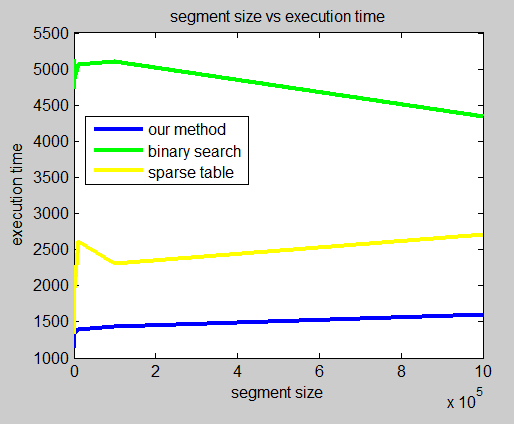
\includegraphics[width=2.3in]{figures/1drandomsmallexec.png} \quad
\subfigure{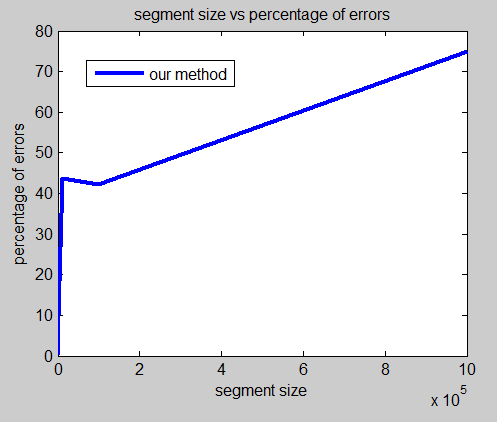
\includegraphics[width=2.3in]{figures/1drandomsmallerr.png} }}}
\caption{1-D: Random segments: Small queries: Exec time and Error percent} \label{randsmall}
\end{figure}

\begin{figure}
%\centering
\mbox{\subfigure{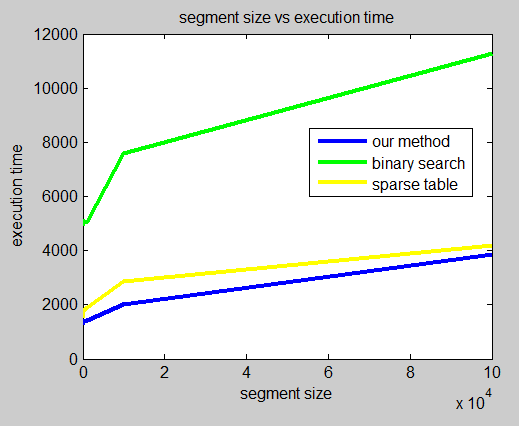
\includegraphics[width=2.3in]{figures/1drandomlargeexec.png} \quad
\subfigure{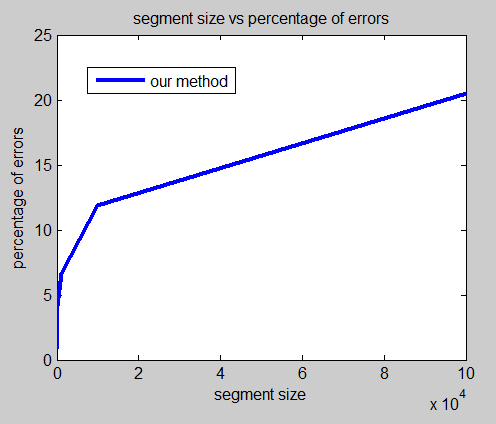
\includegraphics[width=2.3in]{figures/1drandomlargeerr.png} }}}
\caption{1-D: Random segments: Large queries: Exec time and Error percent} \label{randlarge}
\end{figure}

\subsection{Two Dimensional R1Q}
We used a two dimensional input array of size $n_1 = 1000$ (rows) and $n_2$ (columns). The execution time is compared with the naive scan algorithm which is shown in red and our algorithm is shown in blue.

\subsubsection{Random words set to all ones}
In this pattern, some random words are set to all ones. We used $n_2 = 25600$. Figure \ref{2drandones} gives the execution time and error percentage of our algorithm. The number of random words set to all ones are varied from 4K to 240K in increments of 4K. 

The scan algorithm ran faster than our algorithm after a certain point. We see that the error percentage is inversely proportional to the number of words set to all ones.
\begin{figure}
%\centering
\mbox{\subfigure{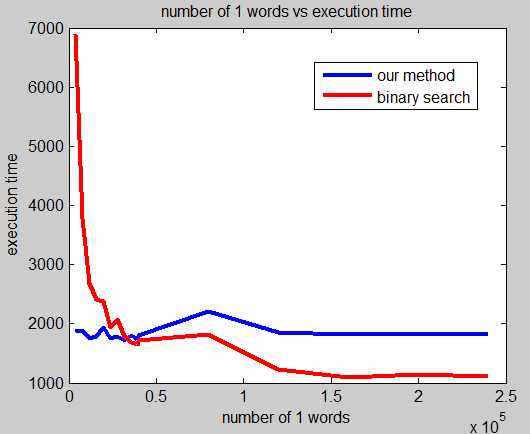
\includegraphics[width=2.3in]{figures/2dallonesexec.png} \quad
\subfigure{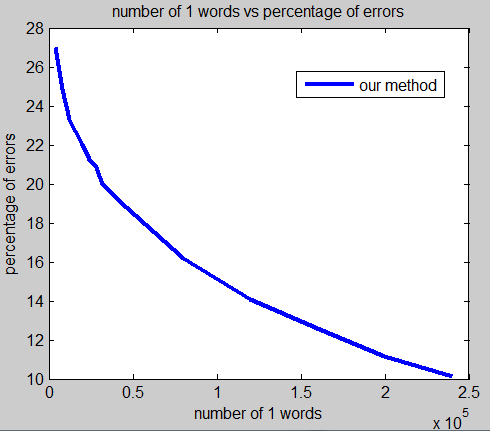
\includegraphics[width=2.3in]{figures/2dalloneserr.png} }}}
\caption{2-D: Random words set to ones: Exec time and Error percent} \label{2drandones}
\end{figure}

\subsubsection{All words set to random numbers}
In this pattern, all the words are set to random numbers. We vary $n_2$ from 128 to 32768 in factors of 2. Figure \ref{2drandom} gives the execution time and error percentage of our algorithm. 

The scan algorithm ran faster than our algorithm. We see that the error percentage is inversely proportional to the number of columns. Also that error percentage is less because of more randomness in the input array.
\begin{figure}
%\centering
\mbox{\subfigure{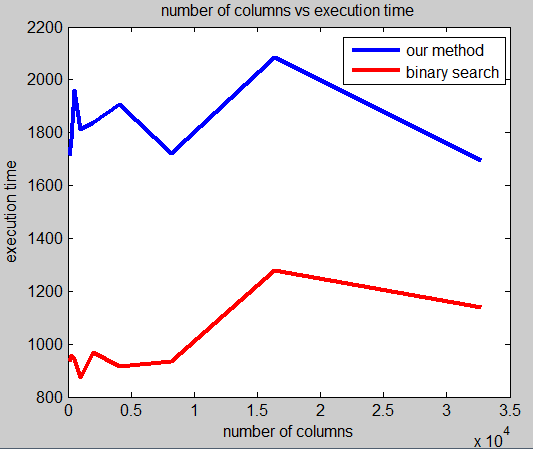
\includegraphics[width=2.3in]{figures/2drandomexec.png} \quad
\subfigure{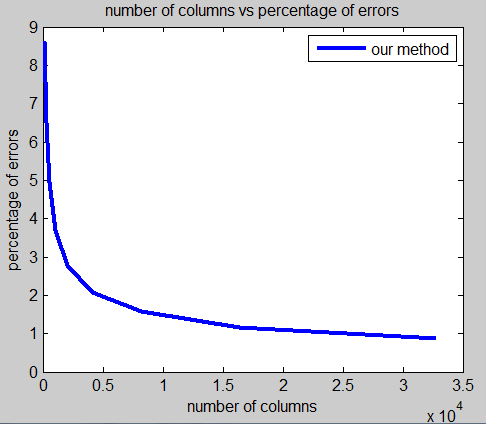
\includegraphics[width=2.3in]{figures/2drandomerr.png} }}}
\caption{2-D: All words set to random numbers: Exec time \& Error percent} \label{2drandom}
\end{figure}

\section{Conclusion}
We surveyed some existing algorithms to solve RMQ problem. Then we proposed an approximation algorithm to solve the 1-D R1Q problem with sublinear space and constant time. The algorithm was later extended to be used in higher dimensions with sublinear space and time as a function of dimensions.

The proposed algorithm was implemented in C++ and the results were plotted. The graphs showed that the algorithm works well with big data and with longer queries. Also, that the algorithm works very well with randomized data set. As the error percentage is less and the space required is very less, the algorithm can be used in different applications.

\bibliographystyle{amsplain}
\bibliography{R1Q}
%\label{lastpage}
\end{document}
